\chapter{Literature Review}
Hypernymy identification and discovery are broadly split into pattern-based and distributional methods \citep{camacho2018semeval, Wang2017}.  The two classes need not be mutually exclusive and we will encounter hybrid methods which integrate features from both approaches, improving on the result achieved by employing each respective method independently  \citep{shwartz2016path, bernier2018crim}.  Despite being overshadowed by distributional methods in recent years, there has been renewed interest in pattern-based methods \citep{roller2018hearst}, a fact that underscores their continued relevance.

\section{Pattern-Based Methods} \label{Pattern-Based Methods}
Lexico-syntactic patterns frequently occurring in language encode the hypernymy semantic relationship between words bound to the patterns.  Such patterns are still referred to as Hearst patterns in tribute to the Marti Hearst's pioneering work on hypernym discovery more than 25 years ago \citep{hearst1992automatic}.

\subsection{Hearst Patterns} \label{Hearst Patterns}
\citeauthor{hearst1992automatic} kick-started the chase for hypernyms when she proposed that the text corpus itself contained information about the language in which it was written \citep{hearst1992automatic}.  She observes that an unknown word within a text can be understood by the reader via word pattern co-occurrences that unambiguously entail the word to a familiar superordinate term \citep{hearst1992automatic}.  Consider the following sentence snippet:

\say{African birds such as turacos, trogons and nicators are…}

The phrasing conveys a semantic \textbf{is-a} relationship between \textit{turacos, trogons and nicators} and the more generic term \textit{bird}.  The compound noun \textit{African bird} is a more specific type of bird and more general than a \textit{turaco} making it a hypernym of \textit{turaco} and hyponym of \textit{bird}.  Anyone reading this excerpt only needs to be familiar with the concept of \textit{bird} to acquire some knowledge of what a \textit{nicator} is.  In the absence of the [Y such as X] syntactic pattern, the sentence contains no other clues on what a \textit{trogon} could mean.  The pattern is also able to expose a co-hyponym relationship between \textit{turacos, trogons and nicators}, all them being a type of bird.  

The variety of free text initially casts doubt on whether representative lexical constructs can be found at all.  Notwithstanding, armed with a few seed examples, Hearst was able to bootstrap a system to automatically acquire six high-quality patterns \citep{hearst1992automatic} from the Grolier’s Academic Encyclopedia digitised corpus \citep{grolier1990academic}:

\begin{itemize}
    \item X [,] and other Y
    \item X [,] or other Y
    \item Y [,] such as X
    \item Y [,] including X
    \item Y [,] especially X
    \item Such Y as X
\end{itemize}

To harvest the patterns, Hearst first collected a list of word-pairs for which the hypernymy relation holds and recorded the textual environment in which the words featured.  High frequency environments were considered predictive of hypernymy and were converted to generalised patterns.  The new patterns were subsequently used to find new seed word-pairs which further fuelled the cycle of pattern discovery \citep{hearst1992automatic}.  Although Hearst focused on English, lexico-syntactic patterns were also induced in a wide variety of languages: Spanish, French, Italian, Dutch \citep{faralli2018misa}; Swedish \citep{rydin2002building} in \citep{sahin2017}; Turkish \citep{sahin2016extraction} in \citep{sahin2017}; and Chinese \citep{Fu2014}.

The pattern-based approach is not necessarily amenable to locate other semantic relations.  Hearst was not able to identify high-yield patterns that identify meronymy \citep{hearst1992automatic}, although more success was observed in languages other than English \citep{sahin2017}.  Hypernymy might be particularly suited to this technique due the classification nature of the relation.  This hypothesis also makes an encyclopedia an ideal corpus from which to extract hypernyms due to the high concentration of definitions within such a text.    This justifies Wikipedia as the corpus of choice in diverse tasks such as taxonomy learning \citep{bordea2016semeval} and linguistic resource construction \citep{Flati2016, Baroni2011}.  

Lexico-syntactic patterns are not entirely resistant to the ambiguity of language.  \citeauthor{wu2012probase} provide several sample phrases where the application of Hearst patterns leads to incorrect hypernyms \citep{wu2012probase}.  \say{Animals other than dogs such as cats…} will result in \(hypernym(cat, dog)\) which is an obvious false positive \citep{wu2012probase}.  Consequently, pattern-based methods sacrifice precision for recall \citep{Wang2017, Snow2004, ritter2009anyway}.  This is exacerbated by the constraint that hyponyms must co-occur with their hypernyms within the scope of a sentence which is not always the case in general-purpose texts.  In the SemEval 2018 Shared Task 9 \citep{camacho2018semeval} English general-purpose corpus, most of the training pairs do not even feature in the same paragraph, much less in the same sentence \citep{bernier2018crim}.


Despite these limitations, Hearst’s early attempt yielded results promising enough to inspire related work.  7,067 sentences contained the construct \textit{such as} contiguously out of the 8.6-million word corpus \citep{grolier1990academic}.  Within these sentences, 152 hypernymy relations were found that adhered to the experiment’s constraints, chiefly that hypernym and hyponymy terms were unmodified.  Similar to later research \citep{kozareva2010semi}, Hearst compares the results of her pattern-mining algorithm with the noun hierarchy featured in an early version of WordNet (1.1) \citep{Miller1995}, which at the time comprised 34,000 noun forms organised into approximately 26,000 \ac{synset}s.  Of the 152 relations, both words in the hyponym/hypernym word-pair were found in WordNet in 106 cases.  61 of these relations were also found to exist in WordNet.  

Fittingly, Hearst was also the first to observe limitations to her approach.  Some mined hypernyms were overly generic (ex. the hypernym \textit{species} does not convey much about the hyponym other than it is a living organism).  In other cases, the context influenced the hypernym to make it too specific; for instance \textit{aircraft} was found to be a \textit{target} because of the military sense of the text in question \citep{hearst1992automatic}.

\subsection{Extending Hearst with Probabilistic Methods}
The examination of the pattern-based methods’ weaknesses was extended by \citeauthor{Wang2017} who note that the absence of “world knowledge” limited the precision of these methods \citep{Wang2017}.   They present other challenges inherent in Hearst Pattern parsing:
\begin{itemize}
    \item Since hypernym and hyponym words are nouns or noun phrases, several named entities will be excluded since they are not considered noun phrases.  For instance: \say{…classic movies such as Gone with the Wind…} where \textit{Gone with the Wind} is actually a proper noun and type of movie (as well as classic movie);
    \item Named entities sometime feature the word \textit{and} in their name.  Examples include \textit{Proctor \textbf{and} Gamble}, \textit{Alf Mizzi \textbf{and} Sons Ltd.}, \textit{Plough \textbf{and} Anchor} etc. A pattern like \say{…companies such as IBM, Nokia, Proctor and Gamble…} will consider \textit{Proctor} and \textit{Gamble} to be two different hyponym candidates;
    \item Co-hyponym lists can contain mixed types.  For example: \say{…representatives in N America, Europe, the Middle East, Australia, Mexico, Brazil, Japan, China, and other countries…} features a mix of continents/regions and actual countries.  A literal interpretation of this pattern would result in \(hypernym(Europe, country)\) which is clearly wrong;
\end{itemize}

\citeauthor{Wang2017} mitigate the ambiguity inherent in pattern-mining by proposing an unsupervised, iterative process that refines the collection of harvested hypernym pairs together with a knowledge dictionary over several epochs, designed to improve both precision and recall \citep{Wang2017}.  The process is broken down into three sub-procedures.  

The Hearst-like patterns are first applied on each sentence of an input corpus text.  Given that they adhere to some imposed constraints, noun phrases are added to a list of potential hypernyms and hyponyms respectively.  All combinations of compound noun phrases such as \textit{Proctor and Gamble} are considered (i.e. \textit{Proctor}, \textit{Gamble}, and \textit{Proctor and Gamble}).  This step generates a list of subordinate words and a list of potential hypernyms for every parsed sentence.  The latter list needs to be reduced to the single, most likely hypernym \citep{Wang2017}.

In the second sub-procedure, conditional probability is used to choose the most likely hypernym from two or more potential superordinate words mined from a single sentence.  The algorithm measures the probability of each candidate word being a hypernym of the collected hyponyms by referring to the knowledge dictionary.  Note that the knowledge dictionary contains high confidence word-hypernym pairs.  The word recording the highest conditional probability $p(y_i | X_s)$, where $y_i$ $\in$ $\{y_1,\ldots,y_n\}$ are candidate hypernyms and $X_s=\{x_1,\ldots, x_m\}$ are collected hyponyms, is chosen as the most likely hypernym in the sentence.  The co-hyponyms in \(X_s\) are assumed to be independent and equally related to the hypernym \citep{wu2012probase}.

The third sub-procedure takes on the mined co-hyponym list and estimates the validity of each of the captured hyponyms.  This step is needed to determine whether conjoined noun phrases (ex. \textit{Proctor and Gamble}) represent separate words or should be taken as an atomic entity.  Another objective of this step is to find the longest sequence of conjoined terms in which co-hyponymy applies, given sentences like \say{… representatives in N America, Europe, the Middle East, Mexico, Brazil, Japan and other countries …}.  In the absence of world knowledge, this mix of continents, regions and actual countries could all be considered \textit{country} subordinates based on the pure application of the Hearst pattern.  With the help of the knowledge dictionary, a similar probabilistic mechanism is employed here too, to determine the likelihood of each of these terms co-occurring with other already-discovered terms linked to the \textit{country} hypernym \citep{wu2012probase}.  

The algorithm produces a set of hypernymy relations which make up the edges of a taxonomy.  The construction of the taxonomy itself falls outside the scope of this dissertation although it is worth noting that the probabilistic framework is extended to the taxonomy’s measure of uncertainty with respect to ambiguous information contained within it.  The algorithm was applied on a massive scale:  326 million sentences were extracted from a corpus composed of 1.7 billion web pages to induce 2.7 million distinct concepts; 16.2 million concept-instance pairs and 4.5 million concept-sub-concept pairs \citep{wu2012probase}.  The result is \textbf{Probase}, a taxonomy comparable in complexity  - measured in terms of the taxonomy’s depth - to WordNet \citep{Miller1995}, YAGO \citep{suchanek2007yago}, and Freebase \citep{bollacker2008freebase}, but an order of magnitude larger.  Probase’s coverage is much wider than Freebase, the only taxonomy comparable in size in terms of concept-instance pairs, with Probase featuring highly-specific concepts such as \textit{celebrity wedding dress designers}\footnote{https://concept.research.microsoft.com/Home/Introduction}.  The top ten Freebase concepts comprise 70\% of its word-instance pairs while only 4.5\% of concept-instance pairs are contained in the top ten concepts of Probase.

\citeauthor{camacho2017we} stated that taxonomies were hard to evaluate automatically \citep{camacho2017we} and Probase was no exception.  Evaluation was estimated manually by human judges who were asked to determine the correctness of 50 randomly selected concept-instance/sub-concept pairs drawn from 40 concepts across a multitude of domains.  The average precision (AP) measured was 92.8\% although no inter-annotator agreement scores were provided.  The AP score was only bettered by YAGO \citep{suchanek2007yago} at 95\%.  \citeauthor{wu2012probase} observe that YAGO is a Wikipedia-based framework which features cleaner sources than the general web corpus that populated Probase \citep{wu2012probase}.  \citeauthor{yu2015learning} used Probase to furnish a large training dataset consisting of 5.8 million hypernym word-pairs, to learn supervised embeddings optimised to detect hypernymy \citep{yu2015learning}.

\subsection{Learning Patterns Automatically} \label{Learning Patterns Automatically}
Although Probase shows that it is possible to harvest a vast number of concepts using Hearst patterns \citep{hearst1992automatic} exclusively, \citeauthor{Snow2004} leveraged machine learning to learn new patterns from a corpus \citep{Snow2004}.  The novelty of their work was the use of a dependency parser (MINIPAR) to examine the grammatical structure of the corpus sentences with the objective to find syntactic relationships between the words.  The dependency path is a directional link between two words composed of the word lemmas or stems, part-of-speech tags and dependency label.  The \ac{POS} tag categorises the word class (noun, verb, adjective, etc.); the dependency label indicates the nature of the link between the words.  Figure~\ref{fig:simple_dep_tree} displays\footnote{https://explosion.ai/demos/displacy} the dependency tree of the sentence \say{A Labrador is a dog}.
\begin{figure}[ht!] % supposedly places it here ...
  \centering
  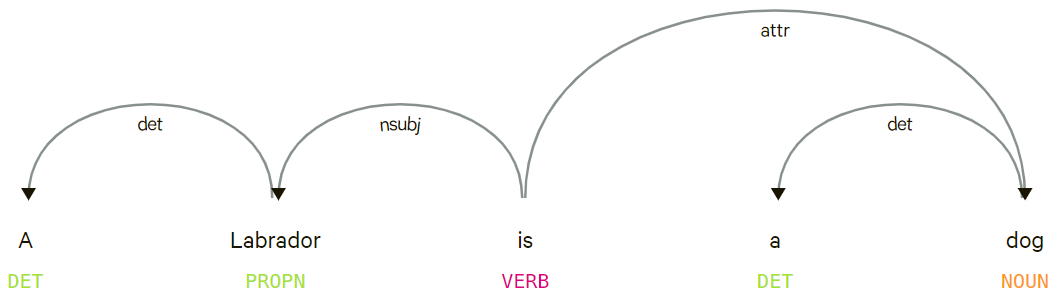
\includegraphics[width=1.\linewidth]{images/dependency_parse.png}
  \caption{Example dependency tree of a simple sentence.\index{Dependency tree}}
  \label{fig:simple_dep_tree}
\end{figure}
The dependency path can be represented as a feature according to a bespoke notation.  An edge between two words can be captured with the tuple $(lemma, pos_tag, dependency_label, direction)$ and the link between two related words expressed as a list of edges.  The link between the hyponym \textit{Labrador} and its hypernym \textit{dog} would be expressed as the sequence:
\[(Labrador, PROPN, NSUB, <), (be, VERB, ROOT, -),(dog, NOUN, ATTR, >)\]

This particular notation is used in \citep{shwartz2016path} which we found more intuitive than the older convention used in \citep{Snow2004}.  To avoid longer, potentially less precise paths, a limit on the links between nouns can be imposed.  \citep{Snow2004} opted for the shortest path consisting of a maximum of four links between any two nouns.

To avoid extreme sparsity in the path vector model, \citeauthor{Snow2004} harvested dependency paths that held for at least five different word pairs from a corpus of 6 million news article sentences \citep{Snow2004}.  Doing so they generated 69,592 distinct dependency path features.  The corpus was also used to extract training and evaluation data.  As \citeauthor{wu2012probase} did later on in \citep{wu2012probase}, \citeauthor{Snow2004} extracted hyponym-hypernym word-pairs from each sentence in their corpus.  Invoking WordNet \citep{Miller1995} as lexical resource, they split the set of pairs into known hypernymy and random words.  To consider a word-pair, both of its constituent words had to be first detected in WordNet.  An ordered word-pair $(x, y)$ would be added to the known hypernym set, if $y$ is found to be an ancestor of $x$.  Words that were not hierarchically related were consigned to the random word list.  The ratio of known hypernyms to random words was 1:50.    

The dataset was used to evaluate the quality of the mined dependency paths.  This was done by applying a simple binary classifier to each path, and predicting hypernymy if a word-pair was connected by a dependency path at least once.  This exercise supplied quantitative support for the efficacy of Hearst’s manually derived patterns, all of which were found to be highly-predictive of hypernymy.  A further four patterns were also found to be high-performing:
\begin{itemize}
    \item $Y$ like $X$;
    \item $Y$ called $X$;
    \item $X$ is a $Y$;
    \item $X$, a $Y$;
\end{itemize}

\subsection{Leveraging Classifiers to Predict Hypernymy}
Intuitively, pattern occurrence frequency should be positively correlated to hypernym detection success.  \citeauthor{Snow2004} create two \ac{VSM}s.  One is a 69,592 dimensional matrix, where each dimension represents a particular dependency path and its value is the total number of times that dependency path connected an input word-pair.  They also create a bucketed, binary vector model where each dependency path corresponds to a 14-dimension “one-hot” encoded binary vector with each dimension capturing the number of pattern occurrences on an exponential scale from 1 (single occurrence) to 8192.  Thus, every word-pair is encoded as a 974,277-dimensional, sparse vector \citep{Snow2004}.  Using the same training set employed to quantify dependency path effectiveness, they train two logistic regression classifiers using each feature vector space respectively.  A significant improvement was observed compared to a simple Hearst pattern-only baseline, which classifies hypernymy if the presence of one or more Hearst patterns is found binding the input word-pair.  Their logistic regression model trained on the bucketed, “one-hot” vectors yields a 0.3480 F1 score, a 132\% improvement over the baseline \citep{Snow2004}. 
\citeauthor{ritter2009anyway}, on the other hand, advocate analysing the word form of the pattern-matched words, prior to proposing them as viable hypernym candidates \citep{ritter2009anyway}.  In particular, words detected in the plural-form by a POS-tagger are more likely to be precise hypernyms when found in certain in patterns \citep{ritter2009anyway}.  They also examine the importance of pattern occurrence frequency in their experiments, focusing on the standard Hearst patterns.  The ambiguity of the English language makes it such that high-frequency patterns alone cannot always guarantee correct hypernyms.  The authors furnish negative hypernymy examples, despite the matching highly-occurring patterns \citep{ritter2009anyway}:
\begin{itemize}
    \item \say{…all around the world including Australia, …} $\Rightarrow$ $hypernym(Australia, world)$
    \item \say{…information about this hotel such as rates, …} $\Rightarrow$ $hypernym(rates, hotel)$
    \item \say{My dog is a bloodhound} $\Rightarrow$ $hypernym(dog, bloodhound)$
\end{itemize}

They distinguish between “left” and “right” patterns where the hyponym $X$ features to the left or right of the hypernym $Y$ in a sentence.  The first two negative examples above are instances of “right” patterns and the last an incorrect instance of a “left” pattern.  \citeauthor{ritter2009anyway} engineer a set of frequency-related features for a given a word-pair.  In addition to total distinct pattern matches, they include features that capture “left” and “right” pattern matches; the total number of times that the hyponym is related to the hypernym via the lemma \textit{be}; the percentage of matches where the hyponym is preceded by an article, determiner or quantifier; the frequency rank of the hypernym with respect to the hyponym in the pair \citep{ritter2009anyway}.   

The word-pair dataset is extracted using TextRunner \citep{banko2007open}, applied on a 117 million web page corpus, which is then validated manually.  A test data-set consisting of 953 pairs is set aside and is split into common concepts (370 pairs) and named entities (583 pairs).  The pattern frequency vector is fed into \textsc{HypernymFinder$_{SVM}$}, a \ac{SVM} classifier \citep{platt1999probabilistic} designed to improve on an earlier na\"ive rules-based classifier that excluded hypernymy in word-pairs that did not match both left and right Hearts patterns.  An \ac{SVM} classifier splits the vector space by estimating hyperplanes which maximise the distance margin between them and the closest training-set samples.    
Unlike \citeauthor{Snow2004} who used WordNet as an evaluation and comparison tool \citep{Snow2004}, \citeauthor{ritter2009anyway} merge WordNet with \textsc{HypernymFinder$_{SVM}$} to create a hybrid classifier.  
Moreover, they opt for a hypernym discovery setup, foreshadowing the SemEval Task 2018 task 9 shared task \citep{camacho2018semeval}.  They retrofit the precision and recall metrics to measure respectively the percentage of overall correct hypermys and the percentage of terms for which one correct hypernym was proposed \citep{ritter2009anyway}.  

WordNet can return high-quality hypernyms but suffers from low coverage, especially with regards to named entities.  Each test candidate was first looked up in WordNet in which 17\% and 64\% of named entities and common nouns respectively were found.  Given some bounded vocabulary (details of which are elusive in their paper), the hybrid classifier outputs the five words it considers most likely to be hypernyms of the test words missing in WordNet.  In this manner, \citeauthor{ritter2009anyway} boosted the WordNet baseline for named entities and, to a lesser extent, common nouns.  Recall/precision increased from 0.17/1.0 to 0.32/0.9 and from 0.64/1.0 to 0.7/0.9 for named entities and common nouns respectively \citep{ritter2009anyway}.  Precision suffers with increased recall since the classifier’s output cannot be of the gold-standard level maintained in WordNet.

\subsection{Identifying Co-hyponyms to Increase Recall}
\citep{Snow2004} and \citep{ritter2009anyway} both acknowledge the limitation of Hearst patterns \citep{hearst1992automatic}.  Most hypernyms simply do not feature in the same sentence with their hyponyms \citep{Snow2004, ritter2009anyway}.  They hypothesise about extending the confines of the sentence for an “orphan” hyponym (i.e. no companion hypernym was found for it in a sentence) by finding co-hyponyms with known hypernyms.  If $(x_i, x_j)$ are two coordinate nouns and $hypernym(x_i, NA)$, $hypernym(x_j, y)$ then we can deduce $hypernym(x_i, y)$.

\citeauthor{Snow2004} experiment with various techniques including: building a distributional similarity vector space model; resorting to WordNet to find co-hyponyms for supported terms; and using high frequency conjunction dependency patterns.  Using the distributional similarity vector space the words can be scored for co-hyponym similarity using the symmetric cosine measure.  A linear combination of the probabilities calculated by the hypernym-only classifier and coordinate classifier increased the $F1$ score by 20\% compared to a hypernym-only classifier on a hand-labelled dataset ($F1$ of 0.3268 and 0.2714 respectively) \citep{Snow2004}.

On the other hand, \citeauthor{ritter2009anyway} were inspired by \textsc{Realm} \citep{downey2007sparse}, which uses \ac{HMM}s to perform type checking in an Information Extraction system, especially if the term in question is sparsely represented in vector space.  In \ac{HMM}s, a hidden stochastic process can only be glimpsed at through another stochastic process that produces a sequence of observations.  No information is known about the model's state but we can assume that there exists some model that can generate the data we're able to observe \citep{rabiner1989tutorial}.  For instance, \textit{Pickerington, Ohio} and \textit{Chicago, Illinois} are both cities but the former will be mentioned much less frequently in a balanced corpus.  Using traditional distributional similarity measures, it is unlikely that \textit{Pickerington} and \textit{Chicago} will be deemed similar since the contexts in which they appear are different.  However given an \ac{HMM} with $n$ hidden states that models the corpus, it is possible that $., Ohio$ and $., Illinois$ were generated by the same hidden states since both terms represent US States \citep{downey2007sparse} in \citep{ritter2009anyway}.

\citeauthor{ritter2009anyway} applied the same concept to finding terms similar to a given hyponym.  To do so, a word is represented by the distribution of the hidden states’ probability of the term being generated by the \ac{HMM} model.  Thus, given an \ac{HMM} model with $n$ states, an $n$-dimensional vector representation is returned.  Similar words to a given term were found by applying a similarity metric on the \ac{HMM}-based feature vector.  The final incarnation of the authors' hypernym finder, is a linear combination of the probability calculated by the \textsc{HypernymFinder$_{SVM}$} classifier and the probability that a given term $x$ has a coordinate word which is a hyponym of the candidate hypernym $y$. Since word similarity alone is tenuous evidence for such words sharing a hypernym, the \ac{HMM} classifier predicts hypernymy in a $(x, y)$ word-pair only if $x'$ exceeds a similarity threshold with $x$, and $x'$ is hyponym of $y$ \citep{ritter2009anyway}.

\subsection{Encoding Dependency Paths with an LSTM}
We have seen that using dependency paths as features can lead to a highly-dimensional vector space.  In one study we have examined, almost 70,000 distinct dependency paths were extracted from a corpus.  Vectors will be sparse since a particular word-pair will only activate a small number of dependency paths.  To improve dependency path representation, \citeauthor{shwartz2016path} trained a \ac{LSTM} \citep{hochreiter1997long} encoder to learn path vectors that are optimised towards detecting hypernymy \citep{shwartz2016path}.  The path vectors are fed into a classifier which predicts whether the dependency pattern feature captures the hypernymy relationship in a given word-pair.  The model is referred to as \textbf{HypeNET} \citep{shwartz2016path}.

The LSTM belong to a family of neural models known as \ac{RNN}s.  Contrary to regular densely-connected networks which require an entire sequence to be presented at once, \ac{RNN}s can be fed the input, one time-step at a time \citep{chollet2017deep}.  A limitation of \ac{RNN}s is their difficulty to recognise signals that come from distant points in a past sequence which does not make them the ideal choice to learn long-term dependencies.  The \ac{LSTM} overcomes this problem because it is a type of recurrent neural network with the ability to learn long-term dependencies.  By having access to the previous time-steps, it is able to build temporal patterns.  Through the use of a special gate composed of a dot product operator and activation function, it can selectively “forget” irrelevant signals whilst retaining information that is more important at the current time-step \citep{chollet2017deep}.  

The motivation behind using the \ac{LSTM} approach is to generalise the lexical-semantic relation between terms that holds in a multitude of contexts.  Prior to feeding them to the \ac{LSTM}, each word-pair is represented by a sequence of dependency paths in which the words co-occur in the corpus.  To be considered, a word-pair needs to co-occur in the corpus and be represented by at least two unique dependency paths.  The path is represented by a list of edge vectors with each edge made up of the concatenation of the embeddings of the lemma, \ac{POS} tag, dependency label and direction.  The dimensionality of the embeddings vary: \citeauthor{shwartz2016path} use 50, 4, 5, and 1 dimension for each respective component \citep{shwartz2016path} although this is not set in stone.  Hyper-parameter tuning on a validation set can help determine the best network configuration.  The \ac{LSTM} should learn which dependency path sequences are predictive of hypernymy while conveniently forgetting those which have no consequence on the semantic relationship \citep{shwartz2016path}.

The weighted-average of the encoded dependency path vectors is computed prior to feeding it to a softmax classifier, trained to minimise cross entropy loss.  The softmax classifier assigns a probability for both the hypernymy and non-hypernymy target labels, which sum up to 1.

\citeauthor{shwartz2016path} compare their novel approach to \citeauthor{Snow2004}'s model \citep{Snow2004} we discussed in section \ref{Learning Patterns Automatically}. The authors train a logistic regression classifier on the 100,000 most information paths chosen using chi-squared feature selection.  On a random data split, the sparse model returns a precision of 0.843 compared to HypeNET’s 0.811 but the latter scores 0.716 recall, a 58\% improvement over \citeauthor{Snow2004}'s model.    

\section{Distributional Model Overview}
%% Need to find out how to type-set Maltese unicode characters
\say{Ghidli ma’ min taghmilha, u nghidlek x’int} is a Maltese expression which means that the company a person keeps says a lot about that person.  The linguist J.M. Firth (1957) cast a similar sentiment to words, saying that a word’s neighbours can divulge much about that word.  This dictum is framed by the Distributional Hypothesis \citep{harris1954distributional} which states that words with similar meaning occur in similar contexts.  

The Distributional Hypothesis is encapsulated in a \ac{VSM} (also referred to as distributional model), a matrix-type data structure which, at its simplest, captures the occurrences of \textit{row} events in \textit{column} contexts. The matrix’s structure in terms of what the rows and columns represent is a design decision and depends on the statistical semantic hypothesis the matrix is supposed to model.  We will briefly discuss the word-context and pair-pattern matrices, the two main types featured in the hypernymy discovery literature.  We also mention the term-document matrix, which we did not encounter in the literature review but which preceded the other two data structures and influenced their development.  The term-context feature is found at the intersection of row and column.  Features can either be expressed as raw frequencies (positive integers including 0) or can be mapped by a weighting function.  In the latter case the frequency value will be a real number.

The objective of a vector space model \ac{VSM} is to convert discrete word symbols into points in higher-dimensional space \citep{turney2010frequency}.  The word symbol does not convey any meaning through its surface form; however, by projecting each word to a multi-dimensional vector, points that are close according to some distance metric will exhibit some form of semantic relatedness.  Conversely, words corresponding to points that are far apart will tend to be weakly related or entirely unrelated \citep{turney2010frequency}.

We will discuss the matrix types in the following section.  We shall borrow the mathematical notation used in \citep{turney2010frequency} as follows:
\begin{itemize}
    \item $\textbf{X}$ will be our matrix which will be made up of $m$ rows and $n$ columns;
    \item $\textbf{X} \in \mathbb{N}^{m \times n}$ if the frequency is unweighted or $\textbf{X} \in \mathbb{R}^{m \times n}$ if we are adopting a frequency weighting mechanism;
    \item $\textbf{x}_{i:}$ will be a row-vector of $n$ elements representing a word $w_i$ in a vocabulary of terms, extracted from a corpus;
    \item $\textbf{x}_{:j}$ will be a column-vector of $m$ elements representing a document, context or pattern depending on the matrix type;
    \item $x_{ij}$ is a scalar value and measures the association between target word $w_i$ and context/pattern/document $c_j$
\end{itemize}    

Most of the elements of $\textbf{X}$ will be set to zero since a word cannot appear in all contexts and each context will correspond to a small percentage of the entire vocabulary.  Such a matrix is referred to as a sparse matrix, which contrasts with a dense matrix which has non-zero values in most of its elements.

\subsection{Mapping Vector Space Models to Semantic Hypotheses}
Word patterns can be statistically examined to understand how humans attribute meaning to the words \citep{turney2010frequency}.  Four main hypotheses were developed, supported by a corresponding mathematical matrix structure that allows each hypothesis to be explored empirically.

\subsubsection{Bag of Words}
According to the bag of words hypothesis \citep{salton1975vector}, we can represent a document in terms of the frequency distribution of the words that compose it.  The term-document matrix is the ideal structure to model this hypothesis.  X will be composed of a vocabulary of m words, extracted from n documents where each row $\textbf{x}_{i:}$ vector is a term word and each column vector $\textbf{x}_{:j}$ is a document.  Thus, the document is represented as a bag of words vector, where each dimension contains the frequency of a word $w_i$ in the document.  In the bag of words model, several aspects of language use are lost, including sequential word ordering, and syntactic links between the words.  Indeed the entirety of the document structure is absent since we cannot tell how the words were strung together in sentences, paragraphs and sections.    Despite these misgivings, the bag of words technique can effectively capture similarity between documents on the basis of word distribution alone \citep{turney2010frequency}.  This result is supported by the intuition that the domain or topic of a document influences the choice of the words used to compose the document \citep{turney2010frequency}.

\subsubsection{Word-context}
The term-document matrix may be an effective tool to measure document similarity or retrieve the most relevant documents to a given query.  However, a document is far too wide to make an ideal context if we are interested in word similarity.  The distribution hypothesis is better served by a word-context matrix.  \citep{lund1996producing} in \citep{turney2010frequency} proposed a window-based context which only considers a number of words before and after a target word.  The $k$ surrounding words of target word $w$ are: $w-k, \ldots, w-1, w+1, \ldots, w+k $.  

The typical context window size is fairly small, consisting of two to five words \citep{roller2014inclusive, santus2014chasing, shwartz2017siege}.  However, wider context windows are also acceptable.  For instance, in \citep{roller2014inclusive}, one of the context windows spanned an entire corpus sentence.

The context windows can be optionally decorated with their direction with respect to a target word \citep{shwartz2017siege}.  In the sentence \textit{The quick brown fox jumped over the lazy dog}, the directional context of the target word $fox$ is $(quick^-, brown^-, jumped^+, over^+)$. In a non-directional window, the left and right context words are indistinguishable.   

Contexts are not necessarily limited to adjacent words; \citep{lin1998information} in \citep{turney2010frequency} and \citep{levy2014dependency} employed dependency-based contexts.  To build their experimental distributional semantic spaces, \citep{shwartz2017siege} considers both parent-daughter and parent-sister neighbours in a dependency tree.

\subsubsection{Pair-pattern}
The term, represented in the matrix row, is no longer a single word but a word-pair and the matrix column feature becomes a doubly-linked pattern which ties the term word-pair together.  We have seen a pair-pattern matrix in action in \citep{Snow2004}.  The term pair is a tuple containing a hyponym and a candidate hypernym.  Tuples can be positive or negative pairs depending on whether the candidate word is an actual hypernym.  The matrix column feature was a dependency path which linked the two words together by the concatenation of edge links in the parse tree and the feature value was the frequency a word-pair matched that particular pattern.

\citep{lin2001discovery} quoted in \citep{turney2010frequency}, propose the extended distributional hypothesis which states that patterns fitting similar pairs tend to have the same semantics.  Conversely, the latent relation hypothesis states that word pairs captured by similar patterns tend to be bound by a similar semantic relation \citep{turney2010frequency}.  \citep{Snow2004} opted for a supervised approach and utilised various classifiers to learn which paths were mostly indicative of hypernymy.  The path feature set they induced included any path that linked at least five distinct nouns pairs extracted from each sentence in the corpus.  

A variant of the pair-pattern matrix is \textbf{TypeDM} \citep{roller2014inclusive}, where a matrix row represents a term word and the context column is a pair consisting of a context word and a syntagmatic relationship that ties the two words together.

\subsection{Feature Weighting}
At its most elemental, each matrix type quantifies the association between a context and a term by counting the occurrences of the term in a particular context \citep{turney2010frequency}, \citep{shwartz2017siege}.  Often, the raw frequencies are adjusted to compensate for the fact that some words convey little information despite their high recurrence in a corpus.  In the bag of words model, the raw frequencies are transformed using the \textbf{\ac{tf-idf}} function family \citep{turney2010frequency}.  This compels a term to score a high weight if its presence in a document is proportional to its scarcity in other documents.

An alternative to \ac{tf-idf} used to weight features in a word-context matrix is \ac{PMI}:
\[PMI(w_i, c_j) = log \Bigg( \frac{p(w_i, c_j)}{p(w_i)p(c_j)} \Bigg) \]
\ac{PMI} measures the log ratio of the joint probability of a word $w_i$ in a context $c_j$ and the product of the marginal probabilities of $w_i$ and $c_j$ \citep{church1990word} in \citep{turney2010frequency, shwartz2017siege}.

If there is an interesting relationship between $w_i$ and $c_j$, then the conditional probability of $w_i$ given $c_j$ is greater than the joint probability of $w_i$ and $c_j$ given that the two are mutually exclusive.  When that is the case, \ac{PMI} returns a positive value.  On the other hand, if $w_i$ and $c_j$ are independent, \ac{PMI} returns a zero value.  If the presence of a particular context decreases the probability of a word co-occurring, then $p(w_i, c_j)$ is smaller than $p(w_i)p(w_j)$ and a negative \ac{PMI} is returned.

A variant of \ac{PMI} is \ac{PPMI} which enforces every matrix element to be positive or zero if a word does not occur in a particular context.  \ac{PPMI} is biased towards rare events \citep{turney2010frequency} but this can be neutralised by the application of \ac{PLMI} which is returned when \ac{PPMI} is multiplied by the co-occurrence frequency of $w_i$ and $c_j$ \citep{evert2008corpora} in \citep{shwartz2017siege}.

\subsection{Building a Vector Space Model}
A pre-processing pipeline is applied to a corpus before it can be transformed into a matrix-based mathematical model.  The pipeline includes tokenisation, normalisation and, optionally, annotation steps \citep{turney2010frequency}.

At first glance, tokenisation of an English corpus may seem like a trivial task since words are conveniently separated by spaces and sentences divided by the full-stop punctuation mark.  A tokeniser must, however, contend with specificities such as hyphenated words, abbreviations, diverse use of punctuation (ex. \textit{can’t}, \textit{isn’t}, etc.) and multi-word phrases that should be treated atomically (ex. \textit{catch fire}, \textit{vice president}, \textit{Daniel Day-Lewis}) .  Pictogram-based languages such as Chinese and Japanese are harder to deal with since words are not separated by spaces to begin with \citep{turney2010frequency}.

Words expressed with different lexicalisations can sometimes have the same meaning.  A chief example is the capitalisation of a word at the beginning of a sentence which does not change the meaning of the word. Normalisation smoothens surface form variation by lower casing and stemming words. Stemming reduces a word to its most generic form which may not be an actual word.  Highly specific word forms can harm recall which is thus augmented by normalisation but only at the expense of precision \citep{kraaij1996viewing} in \citep{turney2010frequency}.

Annotation increases the specificity of a word by decorating it with descriptors such as the part-of-speech tag, word sense tag, and dependency parse labels.  Word sense disambiguation is particularly relevant in the field of hypernymy detection and discovery since disparate meaning is often attributed to identical word forms.  The hypernym of \textit{bank} can either be \textit{incline} or \textit{financial institution} depending on its word sense.  The attachment of more information to a word is expected to increase precision while punishing recall \citep{turney2010frequency}.

We briefly mentioned all the components needed to build a \ac{VSM} from pre-processing to feature weighting.  To find the degree to which $y$ is a hypernym of $x$ in word-pair $(x, y)$, a metric is applied to the vector representation of $x$ and $y$.  The metrics are collectively referred to as unsupervised methods since they are applied without the need of training data.  In the following section we explore unsupervised methods within selected literature.

\section{Unsupervised Methods}
\subsection{Metric Overview}
Unsupervised methods consists of metrics grouped into four categories, each representative of a hypernymy inflected semantic hypothesis.  \citeauthor{shwartz2017siege} furnish us with an exhaustive survey of metrics across all categories which are listed below.  In all descriptions, $\textbf{x}$ and $\textbf{y}$ represent the term word (hyponym) and candidate hypernym feature vector respectively.  A summary of unsupervised measures which can be used to estimate hypernymy simalarity can be seen in Table~\ref{tab:unsupervised_measures}.

%% Table summarising the measures and grouping them by hypothesis needs to come here
\renewcommand{\arraystretch}{1.2} 
\begin{table*}\centering
    \begin{tabular}{@{}ll@{}} \toprule
    \textbf{Metric}              & \textbf{Source} \\ 
    \cmidrule{1-2}
    \multicolumn{2}{c}{Similarity Measures} \\ \cmidrule(lr){1-2}
    $Cosine Similarity$   & \citep{salton1975vector} \\
    $Lin Similarity$      & \citep{lin1998information} \\
    $APSyn$               & \citep{santus2016unsupervised} \\
    \cmidrule{1-2}
    \multicolumn{2}{c}{Inclusional Measures} \\ \cmidrule(lr){1-2}
    $Weeds Precision$     & \citep{weeds2003general} \\
    $cosWeeds$            & \citep{lenci2012identifying} \\ 
    $ClarkeDE$            & \citep{clarke2009context} \\
    $balAPinc$            & \citep{kotlerman2010directional} \\
    $invCL$               & \citep{lenci2012identifying} \\
    \cmidrule{1-2}
    \multicolumn{2}{c}{Informativeness Measures} \\ \cmidrule(lr){1-2}
    $SLQS$                & \citep{santus2014chasing} \\
    $SLQS_{Sub}$            & \citep{shwartz2017siege} \\
    $SLQS_{Row}$            & \citep{shwartz2017siege} \\
    \cmidrule{1-2}
    \multicolumn{2}{c}{Reversed Inclusional Measures} \\ \cmidrule(lr){1-2}
    $Reversed Weeds$      & \citep{shwartz2017siege} \\
    $Reversed ClarkeDE$   & \citep{shwartz2017siege} \\
    \bottomrule
    \end{tabular}
    \caption{Unsupervised Hypernymy Similarity Measures.}\label{tab:unsupervised_measures}
\end{table*}


\subsubsection{Similarity Measures}
Following the distributional hypothesis \citep{harris1954distributional}, similarity measures focus on the symmetric similarities between the hyponym and hypernym.  Cosine similarity is the inner product of the unit-normalised vectors $\textbf{x}$ and $\textbf{y}$, thus placing the onus of similarity on the angle between the vectors.   The cosine metric measures word similarity by the angle between the vectors $\textbf{x}$ and $\textbf{y}$ where acute angles indicate higher similarity.  The Lin measure is the ratio between common contexts and separate contexts of $\textbf{x}$ and $\textbf{y}$.  A high-level explanation of $APSyn$ can be found in \citep{shwartz2017siege} and more details in \citep{santus2016unsupervised}.

\subsubsection{Distributional Inclusional Measures}
A common criticism of the measures based on the distribution hypothesis is that they are not able to discern among various semantic relations \citep{roller2014inclusive}.  A term word’s nearest neighbours will bear some semantic relationship to it but is not guaranteed to be its hypernym. Moreover, the distributional hypothesis fails to acknowledge the asymmetric nature of hypernymy.  Instead, this is better captured by the distributional inclusional hypothesis \citep{geffet2005distributional} which states that the main contexts of the hyponym term are absorbed in the contexts of its hypernym.  According to this hypothesis, plugging in the generic term instead of the specific term in a sentence would not warp the sentence’s meaning.  $Weeds Precision$ \citep{weeds2003general} is an example of an asymmetric metric that computes the weighted inclusion of the contexts of $\textbf{x}$ within the contexts of $textbf{y}$.  Details of the other measures may be found in their respective papers.

$invCL$ \citep{lenci2012identifying} is another example of an inclusional metric which is calculated as the geometric mean of the degree of inclusion of the hyponym’s contexts in the hypernym’s contexts  and the non-inclusion of the hypernym’s contexts into the hyponym’s contexts.


\subsubsection{Distributional Informativeness Measures}
\citeauthor{santus2014chasing} debated the validity of the distributional inclusional hypothesis.  They argue that the distinction between a hyponym and a hypernym lies in the generality of their contexts.  By virtue of their abstract qualities, hypernyms occur in broad contexts.  Their hyponyms, on the other hand, are specific and thus more likely to feature in explicit contexts.  For instance, an animal has general properties of locomotion, feeding and reproduction but only the echidna and platypus will feature in the context of egg-laying mammals.

The distributional informativeness hypothesis is derived from this principal.  $SLQS$ \citep{santus2014chasing} employs entropy to quantify informativeness.  Lower entropy values imply less uncertainty about the outcome of an event.  Hence, the more general the contexts, the lower the probability we can guess the “topic” of reference and the higher the entropy value.  $SLQS$ calculates the reciprocal difference of the median entropy of the top $N$ contexts of hyponym and hypernym vectors.  $SLQS$ is also an asymmetric measure and if $SLQS(x, y)$ yields a positive value, then $\textbf{y}$ is found to be more general than $\textbf{x}$ which is an indicator of hypernymy.  Three further variants of $SLQS$ were first proposed in \citep{shwartz2017siege}.  $SLQS_{Sub}$ is a weakly symmetric version of $SLQS$ evaluated by subtracting the median entropy of a hyponym's top $N$ contexts from the median entropy of its hypernym's top $N$ contexts.  $SLQS_{Row}$ exploits the fact that the context and target word entropies are not highly correlated, thus repositioning $SLQS$ in terms of target word entropy \citep{shwartz2017siege}.  Finally, $SLQS_{Row, Sub}$ uses the same subtraction expression as $SLQS_{Sub}$ on $SLQS_{Row}$.

\subsubsection{Reversed Inclusional Measures}
The distributional inclusional hypothesis is directly challenged by the reversed inclusional measures.  The basis of these measures is the hypernym cannot always replace the hyponym in its contexts due to the high specificity of the latter.  \textit{The mammal climbed into the car} would not be a reasonable alternative for \textit{the man climbed into car} despite the fact that a man is a mammal.  \citep{shwartz2017siege} propose a simple variant of Weeds Precision and ClarkeDE to model this property, consisting of switching the original function parameters around.  Thus $WeedsPrec(x,y)$ becomes $ReversedWeedsPrec(y, x)$ and the same principle applies to ClarkeDE.

\subsection{Application of Unsupervised Metrics in Selected Literature}
In \citep{santus2014chasing},  a 2.7-billion word corpus was constructed by concatenating the ukWaC \citep{ferraresi2007building} and WaCkypedia corpora in English \citep{baroni2009wacky}.  Word context was provided by a two-word window on either side of the target word and \ac{LMI} was used to weight the features.  The BLESS dataset \citep{Baroni2011} was recruited as an evaluation dataset.  Besides providing hypernyms for 200 English concepts, BLESS also features several negative examples of hypernymy which include other semantic relations such meronym, co-hyponymy and randomly unrelated words.

\citeauthor{santus2014chasing} pitted the distributional inclusional and informativeness hypotheses against each other over two tasks.  $WeedsPrec$ \citep{weeds2003general} represents the inclusional metric family while the informativeness hypothesis is represented by $SLQS$ \citep{santus2014chasing}.  The first tasks involves detecting hypernymy in each positive word-pair using the most frequently occurring word as a baseline.  The second, harder task consisted of discriminating hypernymy from the other semantic relations.

\begin{table*}\centering
    \begin{tabular}{@{}lrrrr@{}} \toprule
    \textbf{Metric}  & \textbf{Hypernymy} & \textbf{Co-hyponymy} & \textbf{Meronymy} & \textbf{Unrelated} \\
    \cmidrule{1-5}
    \textit{Baseline}   & $0.40$ & $0.51$ & $0.38$ & $0.17$ \\
    \textit{Cosine}   & $0.48$ & $0.46$ & $0.31$ & $0.21$ \\
    \textit{WeedsPrec}   & $0.50$ & $0.35$ & $0.39$ & $0.21$ \\
    \textit{SLQS $\times$ Cosine}   & $\textbf{0.59}$ & $\textbf{0.27}$ & $\textbf{0.35}$ & $\textbf{0.24}$ \\
    \bottomrule
    \end{tabular}
    \caption{\ac{AP} of two unsupervised metrics when discriminating semantic relations.}\label{tab:santus_comparison}
\end{table*}

$WeedsPrec$ does not beat the baseline in the first task, scoring a precision of $0.6304$ (compared to a $0.6609$ baseline) while $SLQS$ does better, yielding a precision score of $0.87$.  Distributional similarity is leveraged in the second task by assuming that a hypernym observes two rules: the hyponym must be distributionally similar to the hypernym; the hypernym must be more general than the hyponym.  To merge the two, the product of cosine similarity and positive $SLQS$ is computed.  Precision is replaced by \ac{AP} as evaluation metric where \ac{AP} evaluates the ranking of the predicted hypernymy word-pairs against false positives pertaining to other relations.  The results are reproduced in Table~\ref{tab:santus_comparison} from \citet{santus2014chasing}.

$SLQS$ is less likely to confuse co-hyponymy for hypernymy than $WeedsPrec$ which suggests that in general the co-hyponym in the candidate word slot ($y$) is as specific as the query word ($x$).  The scores reflect the average precision over all 200 concepts in the BLESS dataset ($AP@all$).

In \citep{shwartz2017siege}, the authors undertake a more ambitious study of unsupervised metrics over four commonly-used datasets: BLESS \citep{Baroni2011}; EVALution \citep{santus2015evalution}; Lenci/Benotto \citep{benotto2015distributional}; and Weeds \citep{weeds2014learning}.  Each dataset features positive hypernymy examples and negative examples consisting of words that are related together via some other semantic relationship such as meronymy, synonymy, co-hyponymy or randomly unrelated.  The study tests each metric’s ability at distinguishing hypernymy from the other relations.  Furthermore, experiments were also carried out to measure the metric’s performance at detecting hypernymy among specific relations in isolation. 

\begin{table*}\centering
    \begin{tabular}{@{}cccc@{}} \toprule
    \textbf{Context Type} & \multicolumn{2}{c}{\textbf{Context Parameters}} & \textbf{Feature Weighting} \\ \cmidrule{1-4}
    \multirow{6}{*}{Window} & 
    \multirow{3}{*}{Directional} &
    \multirow{3}{*}{$win2d$ or $win5d$} & Raw Freq \\
    & & & PPMI \\
    & & & LMI \\ 
    \cmidrule{2-4}
    & \multirow{3}{*}{Non-Directional} &
      \multirow{3}{*}{$win2$ or $win5$} & Raw Freq \\
    & & & PPMI \\
    & & & LMI \\ 
    \cmidrule{1-4}
    \multirow{3}{*}{Dependency} & 
    \multirow{3}{*}{-} &
    \multirow{3}{*}{$dep$ or $joint$} & Raw Freq \\
    & & & PPMI \\
    & & & LMI \\
    \bottomrule
    \end{tabular}
    \caption{Vector Space Model combinations used in \citep{shwartz2017siege}.}\label{tab:siege_vector_spaces}
\end{table*}

Following \citep{santus2014chasing}, \citeauthor{shwartz2017siege} make use of the same concatenated corpus but in contrast to \citeauthor{santus2014chasing}, lemmatised it and annotated it with part-of-speech tags and dependency labels.  The \ac{VSM}’s vocabulary was limited by only considering nouns, verbs and adjectives that featured 100 times or more in the corpus.  Several \acl{VSM}s were constructed in an attempt to determine which particular combination, in tandem with an unsupervised metric, works best at identifying hypernymy among several relata.  

Table~\ref{tab:siege_vector_spaces} illustrates the \ac{VSM} variants tested.  The authors tested window and dependency-based contexts, with the association between the words and their contexts weighted by raw frequency, \ac{PPMI}, and \ac{PLMI} for a total of 18 matrix combinations. $win2$ and $win5$ represent a two and five word non-directional context window respectively, whereas the $d$ suffix denotes a directional context.  The dependency-based contexts are denoted by $dep$ and $joint$, where the former represents parent-daughter context and the latter captures parent-sister pairs in the dependency tree.

\begin{table*}\centering
    \begin{tabular}{@{}lccccr@{}} \toprule
    \textbf{Dataset} & \shortstack{\textbf{Hyper vs.} \\ \textbf{Relation} } & \textbf{Measure} & \shortstack{\textbf{Context} \\ \textbf{Type} } & \shortstack{\textbf{Feature} \\ \textbf{Weighting}} & \textbf{AP@100} \\ \cmidrule{1-6}
    \multirow{5}{*}{EVALution} & 
    All Relations & $invCL$ & joint & freq & 0.661 \\
    & Meronym & $APSyn$ & joint & freq & 0.883 \\
    & Attribute & $APSyn$ & joint & freq & 0.880 \\
    & Antonym & $SLQS_{Row}$ & joint & freq & 0.740 \\
    & Synonym & $SLQS_{Row}$ & joint & freq & 0.830 \\
    \cmidrule{1-6}
    \multirow{5}{*}{BLESS} & 
    All Relations & $invCL$ & win5 & freq & 0.540 \\
    & Meronym & $SLQS_{Sub}$ & win5d & freq & 1.000 \\
    & Coordinate & $SLQS_{Sub}$ & joint & freq & 0.995 \\
    & Attribute & $SLQS_{Sub}$ & dep & PLMI & 1.000 \\
    & Event & $APSyn$ & dep & freq & 1.000 \\
    \cmidrule{1-6}
    \multirow{3}{*}{Lenci/Benotto} & 
    All Relations & $APSyn$ & joint & freq & 0.617 \\
    & Antonym & $APSyn$ & dep & freq & 0.861 \\
    & Synonym & $SLQS_{Row, Sub}$ & joint & PPMI & 0.948 \\
    \cmidrule{1-6}
    \multirow{2}{*}{Weeds} & 
    All Relations & $ClarkeDE$ & win5d & freq & 0.911 \\
    & Coordinate & $ClarkeDE$ & win5d & freq & 0.911 \\
    \bottomrule
    \end{tabular}
    \caption{Best unsupervised results accompanied by VSM features in comprehensive experiment.}\label{tab:siege_unsupervised_results}
\end{table*}

For each measure, context-type, feature weighting function, the word-pairs were ranked in descending order of the score achieved.  The \ac{AP} was measured in two instances: on the full list of word-pairs; and on the 100 most confidently scored pairs.  A table reflecting the best $AP@100$ results recorded in the experiments is shown in Table~\ref{tab:siege_unsupervised_results} from \citet{shwartz2017siege}.

Results suggest that there does not exist one combination of measure and semantic space that outperforms the rest across the board.  Supported by the best results, the authors speculated that syntactic contexts (dependency, joint-dependency) have higher hypernymy predictive power due to them capturing both proximity and syntactic features.  The na\"ve raw frequency feature weight acquitted itself surprisingly well considering it does not provide more information than co-occurrence of word and context.

The nature of the word-pairs in the datasets influenced the experiments’ outcome and shed some light on why some metrics fared better on some datasets than others.  $SLQS$ outputs a high score if the candidate word being tested for hypernymy is found to be more general than the query word \citep{santus2014chasing}.  It performed well (although not necessarily the best) in the hypernymy/antonymy, hypernymy/synonymy challenges where the (negative) candidate antonyms and synonyms were largely less general than the hypernyms in the set.  Conversely, the symmetric similarity measures were best suited to distinguish hypernymy from words which have few shared contexts.  For instance, the attribute words featured in BLESS are adjectives which share few contexts with the noun term word.  

Like \citep{santus2014chasing}, $SLQS$ was more effective at recognising hypernymy than inclusion-based methods, even when applied onto dependency-based context types.  However, inclusion-based methods such as $ClarkeDE$, $invCL$ and $WeedsPrec$ were superior to $SLQS$ on the Weeds dataset.  \citeauthor{shwartz2017siege} conclude that this result is due to the distribution of words in Weeds, in which every positive and negative hypernym instance features only once.  BLESS contains several repeated hypernyms which, moreover, tend to be rather general (ex. \textit{animal}, \textit{object}).  This plays to the strengths of $SLQS$ which justifies its dominance on this particular set.

\subsection{Criticism of Unsupervised Methods}
We examined empirical work which illustrated the power of unsupervised metrics, founded as they are on sound linguistic hypotheses.  Although the metrics have been used in a hypernymy detection context, they can be leveraged to discover hypernyms by finding the nearest neighbours of a hyponym vector in a particular vector space according to an asymmetric measure based on the distributional inclusional or informativeness hypothesis like the baselines created by the SemEval 2018 Task 9 organisers \citep{camacho2018semeval}.  For unsupervised methods to be effective in this regard, the score returned when considering a hypernymy word-pair must be statistically distinguishable from the score returned if the word-pair is random or linked by some other semantic relation.  Otherwise recognising hypernyms using such methods is reduced to a game of chance.  Although \citep{santus2014chasing} challenged the soundness of inclusion measures, \citep{roller2014inclusive} tested whether asymmetric metrics based on the inclusional hypothesis are able to fulfill this requirement and, unfortunately, found them initially lacking.

\citeauthor{roller2014inclusive} construct a corpus in a manner similar to \citep{santus2014chasing}, but enlarged by the inclusion of Gigaword and BNC.  The authors pre-processed the corpus by lemmatising it and annotating the part-of-speech tags, after which they filtered out words which occurred less than 500 times.  They constructed three vector spaces, two of which were based on a window context (2 words around the target word, and a full sentence respectively), and one based on a TypeDM tensor model.  The vector spaces are denoted as \textit{U+W2}, \textit{U+Sent} and \textit{TypeDM} respectively.  The features of the two window-based models were transformed by \ac{PPMI}.

\begin{figure}[ht!] 
  \centering
  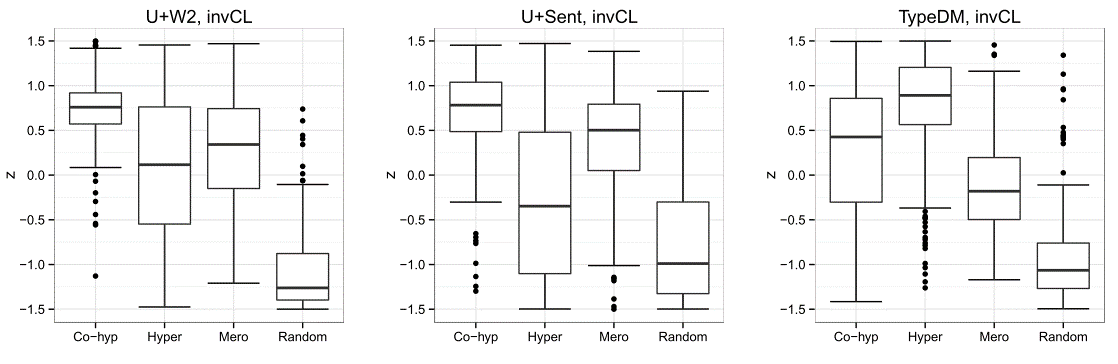
\includegraphics[width=1.\linewidth]{images/standardised_distribution_invCL.png}
  \caption{Standardised distribution of $invCL$ score across relations and VSMs.}
  \label{fig:standardised_invCL_boxplot}
\end{figure}


A battery of inclusional measures, including $WeedsPrec$ \citep{weeds2003general} and $invCL$ \citep{lenci2012identifying}, were used to score the word-pairs in the BLESS dataset \citep{Baroni2011} in each vector space which, as we have already seen, consists of word-pairs tied by several semantic relations.  The scores were standardised and a box-plot of the score achieved when measuring $invCL$ asymmetric similarity - chosen for the best results attained in the experiment - across relations and vector spaces is reproduced in Figure~\ref{fig:standardised_invCL_boxplot} from \citet{roller2014inclusive}.

Despite $invCL$ was the most productive metric at hypernym identification, we can see that performance is not robust across all vector space models.  The standardised $z$-score was significantly higher for hypernymy word-pairs in the \textit{TypeDM} space but was entirely deprived of predictive ability in the \textit{U+W2}  and \textit{U+Sent} \ac{VSM}s. \ac{AP} results for hypernymy against co-hyponymy, meronymy and random relation respectively, depict a similar picture.  In all vector spaces except \textit{TypeDM}, both the asymmetric measures as well as the baseline cosine symmetric measures assigned the highest ranking to co-hyponym terms by a significant margin.  In \textit{TypeDM}, $invCL$ acquires a higher mean average precision for hypernyms than for co-hyponyms but the difference is not statistically significant \citep{roller2014inclusive}.

These experiments pose a conundrum for unsupervised methods research: they have been shown to be successful in some settings but clearly miss the mark in others.  \citeauthor{roller2014inclusive} argued that the distributional inclusional hypothesis was selective and did not apply on all contexts.  However, unsupervised methods of distributional inclusion considered all contexts equally, which ultimately harms their performance \citep{roller2014inclusive}.  They propose a technique similar to \citep{Snow2004}, which leverages a supervised classifier to both learn the distributional signals most associated with a given set of hypernymy word-pairs, and interpret the trained models to understand which features are contributing to the estimated result.

\section{Supervised Methods}
High-quality, ground-truth data and associated target discrete labels (or continuous values if the task is of the regression type), distinguish supervised methods from the unsupervised measures we have reviewed so far.  In the hypernymy identification domain, supervised methods are not grounded in a linguistic hypothesis but attempt to learn the asymmetric metric from a provided training set \citep{levy2015supervised}.

Just like in the unsupervised context, the query and candidate hypernym terms are represented by vectors sourced from a vector space model.  Instead of applying distributional hypotheses, the vectors representing the words in the pair are combined by a vector operations like concatenation \citep{baroni2012entailment}, or difference \citep{roller2014inclusive}.  In the concatenation case, the hypernym vector is added to the tail of the hyponym vector to create a feature which has twice the number of dimensions as the individual word vector.  In the diff case, the hypernym vector is subtracted from the hyponym \citep{roller2014inclusive} or vice versa \citep{shwartz2017siege}.  The combined feature vectors are fed into a classifier together with the target labels.  The literature we reviewed shows a preference for the logistic regression \citep{roller2014inclusive, shwartz2017siege, levy2015supervised, yamane2016distributional, bernier2018crim} and \ac{SVM} classifiers \citep{shwartz2017siege, levy2015supervised, baroni2012entailment}.

\subsection{Classifier Background}
\subsubsection{Logistic Regression}
Despite the name, logistic regression is actually a binary classification learning algorithm that uses the properties of the logistic function $\sigma(z)=\frac{1}{1 + e^{-z}}$ that maps real valued inputs to values between $0$ and $1$.  Values in this range can be interpreted as a probability. The real value input is a linear combination of $m$ features and $m+1$ weights.  This can be expressed in the terms of the logit function: \[logit(p(y = 1 | x)) = z = \textbf{w}^T\textbf{x}\]

The resulting real value can be mapped to a probability using the defined logistic equation.  To learn the best weights (or coefficients) a cost function is required to minimise the error when predicting hypernymy.  This is done by minimising the logistic loss function: 
\[J(w) = \sum_{i=1}^{n}\Big[-y^{(i)}log\big(\sigma(z^{(i)})\big) - \big(1 - y^{(i)}\big) log\big(1-\sigma(z^{(i)}\big)\big)  \Big] \] 

The linear model for binary classification can be extended to the multiclass classification via the \textit{OvR} (one vs rest technique) or using multiclass settings that optimise the model for multi label classification.  Deviations from the correct prediction push the cost function towards infinity thus penalising poor predictions. 

Various gradient descent solvers can be used to minimise the cost function but some are better suited than others depending on the circumstances.  Adam \citep{kingma2014adam} is a sophisticated version of the standard \ac{SGD} solver which attempts to minimise the task’s cost function by taking tiny steps in the direction opposite to the gradient calculated from the cost function’s derivative.  Adam is distinguished from vanilla \ac{SGD} by managing an adaptive learning rate for every trainable parameter.  It is known to work well in several empirical scenarios and is used extensively in the literature we reviewed \citep{shwartz2016path, bernier2018crim, yamane2016distributional, espinosa2016supervised}.

Two problems afflict all machine learning algorithms: bias and variance.  High bias means that the model does not learn enough from the training data, under-fitting the data and does not generalise well to unseen instances.   High variance is when the model misinterprets random noise in the data as important features which do not carry over to new unseen instances.  Variance and bias in logistic regression models can be tuned with the addition of regularisation parameters that penalise extreme feature coefficients. $L2$ regularisation penalises large weights whereas $L1$ encourages sparse solutions – weight coefficients set to $0$, thus nullifying the effect of the corresponding feature on the model.  Because of this reason, $L1$ regularisation is often used as a feature selection technique.

\subsubsection{Support Vector Machines}
%% to be added

\subsection{Representative Work}
\citeauthor{baroni2012entailment}'s work \citep{baroni2012entailment} is considered a baseline in the literature under review \citep{shwartz2017siege, shwartz2016path, camacho2017we, roller2014inclusive, levy2015supervised}.  The study focused on two tasks, but we shall ignore the second task which is related to learning quantifying determiners (ex. \textit{few} entails \textit{some}).  

In the first task, the authors wanted to capture training data for an entailment recogniser by leveraging properties of adjective-noun (AN) composite expressions, such as \textit{red car}.  Based on the fact that most ANs imply the headword noun (\textit{white cat} entails \textit{cat}), the vector equivalent of these pairs can be used to train a classifier to detect hypernymy for other nouns (\textit{cat} entails \textit{animal}).  Like hyponyms, adjective-noun phrases are more specific than the noun and hence their contexts are a subset of the context of the modified noun. 

Corpus pre-processing steps mirror what we have already described in other work.  The author uses a sentence wide word-window context and the features were transformed by \ac{PMI}.  A sparse vector space model composed of $48,000$ target word vector rows and $27,000$ context word columns.  To counter the matrix’s sparsity and improve computation efficiency, the vector was reduced to $300$ components via an \ac{SVD} transformation.  The training data set, partially generated from BLESS, included $1,246$ positive $(AN, N)$ pairs.  Negative instances were induced automatically by linking ANs with randomly-selected nouns in the dataset.  The test set, which had to be composed of (hyponym, hypernym) pairs, was culled from WordNet \citep{Miller1995}, avoiding hypernyms which are too abstract (ex. \textit{object}, \textit{entity}, etc.).  Negative instances were generated using the same method employed in the training set.  

To build the feature vector, \citeauthor{baroni2012entailment} concatenated the vector equivalent of each training pair component together.  Since the vector space was reduced to $300$ dimension, each feature was composed of a $600$-dimension vector.  The author opted for an \ac{SVM} with polynomial kernel to learn the entailment signal.  They supported their choice by noting that a non-linear \ac{SVM} extracts feature interactions automatically, which would otherwise have had to be handcrafted in order to be exploited by a linear classifier like a logistic regression model.  They trained their \ac{SVM} on the $(AN, N)$ pairs and achieved a $69.3\%$ accuracy score when they evaluated the model on the hypernymy test set.  Accuracy ascended to $88.6\%$, when they trained the \ac{SVM} directly on the hypernymy set with $10-$fold cross-validation.  The results showed that a model trained to recognise the head noun in adjective-noun pairs can be effectively transferred to the related - but different - task of distinguishing hypernyms from random words.

\citeauthor{roller2014inclusive} use vector difference to construct their features.  Inspired by the success of \citeauthor{mikolov2013distributed} at using vector subtraction to learn word analogies \citep{mikolov2013distributed}, they come up with their own vector difference variant.  They represent each word-pair by the difference of the unit-normalised vectors, combined with their square differences.  

These features are intended to capture both the dimensions that strongly predict hypernymy and the dimensions that are predictive of random words.
The authors construct a vector space with a sentence wide word-window similar to \citep{baroni2012entailment}.  The corpus used by \citep{roller2014inclusive} differs from \citep{baroni2012entailment} only by the inclusion of Gigaword in addition to BNC, ukWaC and WaCkypedia.  The resultant vector space is reduced to $300$ dimensions by \ac{SVD}, once again mirroring \citeauthor{baroni2012entailment}'s setup.  

The training data were provided by the BLESS and ENTAILMENT datasets.  Instead of splitting the datasets into training and test, they opt to measure the classifier’s ability at identifying hypernyms on all terms in the sets.  To do so, they holdout one term and train on the remaining terms.  Additionally, they carry out a lexical split whereby they ignore any word-pairs in the training set which overlaps one of the words in the test, irrespective of position.  An average accuracy score of $0.80$ and $0.82$ is achieved on BLESS and ENTAILMENT respectively, considerably beyond the most frequent class baseline of $0.46$ and $0.50$ respectively.  \citeauthor{roller2014inclusive} also train an \ac{SVM} classifier on concatenated features and experiment with a variety of vector spaces, achieving similar results.  However, the logistic regression model trained on $diff$ features beat the \ac{SVM} in every experiment attempted.  For the sake of comparison, we specifically mention the result attained on the experiment which was, in our view, most similar to \citep{baroni2012entailment}.



